% ======================================================================
%  Cyber Security - Theory CA-2 (Part 2) - Unit 4 Case Study Report
%  Compile with XeLaTeX  (Overleaf: Menu -> Compiler -> XeLaTeX)
% ======================================================================
\documentclass[12pt,a4paper,oneside]{article}

% ---------------- EDIT YOUR GROUP DETAILS HERE ----------------
\newcommand{\groupno}{G\_\_}            % e.g. G10
\newcommand{\memberA}{Member 1 Name}    \newcommand{\prnA}{PRN}
\newcommand{\memberB}{Member 2 Name}    \newcommand{\prnB}{PRN}
\newcommand{\memberC}{Member 3 Name}    \newcommand{\prnC}{PRN}
\newcommand{\memberD}{Member 4 Name}    \newcommand{\prnD}{PRN}
% --------------------------------------------------------------

\usepackage{fontspec}
\usepackage{unicode-math}
\IfFontExistsTF{Times New Roman}{\setmainfont{Times New Roman}}{\IfFontExistsTF{Liberation Serif}{\setmainfont{Liberation Serif}}{\setmainfont{TeX Gyre Termes}}}
\IfFontExistsTF{TeX Gyre Termes Math}{\setmathfont{TeX Gyre Termes Math}}{}
\IfFontExistsTF{DejaVu Sans Mono}{\setmonofont{DejaVu Sans Mono}[Scale=0.82]}{}
\usepackage{amsmath}
\usepackage[margin=2.5cm]{geometry}
\usepackage{setspace}\setstretch{1.15}
\usepackage{xcolor}
\definecolor{rblue}{RGB}{23,62,140}
\definecolor{lblue}{RGB}{225,234,248}
\definecolor{mblue}{RGB}{143,179,232}
\usepackage{graphicx,float,booktabs,tabularx,multirow,makecell,array}
\usepackage[font=small,labelfont={bf,color=rblue}]{caption}
\usepackage[inline]{enumitem}\setlist{itemsep=2pt,topsep=4pt}
\usepackage{microtype}
\emergencystretch=3em
\usepackage{titlesec}
\titleformat{\section}{\Large\bfseries\color{rblue}}{\thesection.}{0.6em}{}[{\color{rblue}\titlerule[0.8pt]}]
\titleformat{\subsection}{\large\bfseries\color{rblue}}{\thesubsection}{0.6em}{}
\titleformat{\subsubsection}{\normalsize\bfseries\itshape\color{rblue}}{\thesubsubsection}{0.6em}{}
\titlespacing*{\section}{0pt}{14pt}{8pt}
\usepackage{fancyhdr}
\pagestyle{fancy}\fancyhf{}
\fancyhead[L]{\small\color{rblue}Cyber Security -- Unit 4 Case Study}
\fancyhead[R]{\small\color{rblue}Group \groupno}
\fancyfoot[C]{\small\thepage}
\renewcommand{\headrulewidth}{0.4pt}
\renewcommand{\headrule}{\hbox to\headwidth{\color{rblue}\leaders\hrule height \headrulewidth\hfill}}
\usepackage[ruled,vlined,linesnumbered]{algorithm2e}
\SetAlFnt{\small}\SetKwComment{tcp}{$\triangleright$ }{}
\usepackage{listings}
\lstset{basicstyle=\ttfamily\small,keywordstyle=\color{rblue}\bfseries,commentstyle=\color{rblue}\itshape,
  stringstyle=\color{black},frame=single,rulecolor=\color{rblue},backgroundcolor=\color{lblue!45},
  breaklines=true,columns=fullflexible,xleftmargin=4pt,xrightmargin=4pt,showstringspaces=false,
  numbers=left,numberstyle=\tiny\color{rblue}}
\usepackage{tikz}
\usetikzlibrary{arrows.meta,positioning,fit,calc,shapes.geometric}
\usepackage{tcolorbox}
\tcbuselibrary{skins}
\newtcolorbox{keybox}[1]{colback=lblue!50,colframe=rblue,fonttitle=\bfseries,title=#1,boxrule=0.8pt,arc=2pt}
\usepackage[numbers,sort&compress]{natbib}
\usepackage[colorlinks=true,linkcolor=rblue,citecolor=rblue,urlcolor=rblue]{hyperref}
\usepackage{url}
\newcolumntype{Y}{>{\raggedright\arraybackslash}X}
\renewcommand{\textsc}[1]{{\small\MakeUppercase{#1}}}
\newcommand{\hl}[1]{\textbf{\color{rblue}#1}}
\renewcommand{\arraystretch}{1.18}

\begin{document}
% ============================ COVER PAGE ============================
\begin{titlepage}
\thispagestyle{empty}
\begin{tcolorbox}[enhanced,colback=white,colframe=rblue,boxrule=1.6pt,arc=0pt,height=\textheight,valign=top,left=14pt,right=14pt,top=10pt]
\centering
{\large\bfseries\color{rblue} SYMBIOSIS INSTITUTE OF TECHNOLOGY, PUNE}\\[2pt]
{\normalsize Symbiosis International (Deemed University)}\\[14pt]
{\large\bfseries Cyber Security -- Theory CA-2 (Part 2)}\\[2pt]
{\normalsize Case Study Report \;|\; Syllabus: Unit 4}\\[16pt]
{\color{rblue}\rule{0.9\linewidth}{1pt}}\\[10pt]
{\LARGE\bfseries\color{rblue} ForenSight: A Forensic-Ready Hybrid\\[4pt] Intrusion Detection Framework}\\[10pt]
{\large Integrating Signature Rules, Explainable Machine Learning\\ and Tamper-Evident Evidence Logging}\\[10pt]
{\color{rblue}\rule{0.9\linewidth}{1pt}}\\[18pt]

{\Large\bfseries Group Number: \color{rblue}\groupno}\\[16pt]

\begin{tabular}{>{\centering\arraybackslash}p{1.2cm} >{\raggedright\arraybackslash}p{7.2cm} >{\centering\arraybackslash}p{4.2cm}}
\toprule
\textbf{\textcolor{rblue}{Sr.}} & \textbf{\textcolor{rblue}{Name of Student}} & \textbf{\textcolor{rblue}{PRN}} \\ \midrule
1 & \memberA & \prnA \\
2 & \memberB & \prnB \\
3 & \memberC & \prnC \\
4 & \memberD & \prnD \\ \bottomrule
\end{tabular}\\[18pt]

\begin{tabular}{>{\raggedleft\arraybackslash}p{4.4cm} >{\raggedright\arraybackslash}p{9.2cm}}
\textbf{Topic Selected:} & Forensic-ready hybrid intrusion detection (IDS + Malware Analysis + Digital Forensics + Dark-web threat context) \\[4pt]
\textbf{Unit 4 Topics Covered:} & Intrusion Detection Systems, Malware Analysis, Digital Forensics, Dark Web \\[4pt]
\textbf{Faculty:} & Dr.\ Pooja Bagane, Dr.\ Jitendra Rajpurohit \\[4pt]
\textbf{Submission Date:} & Saturday, 10 October 2026 \\
\end{tabular}
\vfill
{\small\color{rblue} All experiments in this report were executed by the group on the public NSL-KDD benchmark;\\ every number reported is reproducible from the accompanying code (random seed = 42).}
\end{tcolorbox}
\end{titlepage}

% ============================ ABSTRACT ============================
\section*{\color{rblue}Abstract}
\addcontentsline{toc}{section}{Abstract}
Intrusion Detection Systems (IDS) are usually judged by a single question---\emph{did the alarm fire?}---yet, after a breach, investigators must also answer \emph{why} it fired and \emph{whether the alert record can be trusted as evidence}. This case study designs, implements and evaluates \hl{ForenSight}, a three-tier hybrid IDS that combines (i) a Snort-style signature engine of twelve rules mapped to MITRE ATT\&CK techniques, (ii) a gradient-boosted (XGBoost) supervised classifier explained per-alert with SHAP values, and (iii) an Isolation-Forest anomaly detector trained only on benign traffic to catch previously unseen (``zero-day'') attacks. Every alert is written to a forensic-ready evidence log in which records are SHA-256 hash-chained and periodically sealed with HMAC anchors, following the preservation and documentation phases of NIST SP 800-86. Evaluated on the NSL-KDD benchmark, whose test set contains 17 attack types absent from training, the hybrid reached \hl{87.2\% accuracy and an F1-score of 0.878} on KDDTest+ at a 3.9\% false-positive rate, compared with 79.2\% / 0.782 for the best single classifier (XGBoost). On the harder KDDTest-21 subset, accuracy rose from 60.4\% to \hl{75.9\%}, and recall on novel attack types increased from 37.0\% to \hl{62.2\%}. In 1{,}000 randomised tampering trials (modification, deletion, re-ordering, full re-hashing and truncation), the evidence log detected \hl{100\%} of manipulations, at a cost of 142\,\textmu s and roughly 402 bytes per alert. The study shows that detection accuracy, explainability and evidential integrity can be engineered together, and it discusses the remaining blind spots (for example SNMP-based attacks that are indistinguishable from normal traffic) that point to future work.

\vspace{6pt}
\noindent\textbf{\textcolor{rblue}{Keywords:}} Intrusion Detection System; Hybrid IDS; Anomaly Detection; XGBoost; Isolation Forest; Explainable AI (SHAP); Digital Forensics; Forensic Readiness; Tamper-Evident Logging; Hash Chain; Malware Analysis; MITRE ATT\&CK; Dark Web; NSL-KDD.

\vspace{8pt}
{\hypersetup{linkcolor=black}\setstretch{1.0}\small\tableofcontents}
\newpage

% ============================ 1. INTRODUCTION ============================
\section{Introduction}
\subsection{Background and Relevance in Today's World}
Cyber attacks against Indian organisations have grown sharply. The Indian Computer Emergency Response Team (CERT-In) handled 11.58 lakh cyber security incidents in 2020; this rose to 15.92 lakh in 2023 and to \textbf{20.41 lakh in 2024}, as reported to Parliament by the Ministry of Electronics and IT \cite{certin2025rs}. Globally, the 2025 Verizon Data Breach Investigations Report analysed 12{,}195 confirmed breaches. It found that exploitation of vulnerabilities was the initial access vector in 20\% of them, a 34\% year-on-year rise, and that ransomware was present in 44\% \cite{verizon2025}. IBM's 2025 \emph{Cost of a Data Breach} study puts the average breach at USD 4.44 million and the average time to identify and contain one at 241 days \cite{ibm2025}. Much of this cost comes from detecting attacks late and reconstructing them poorly.

At the same time, regulation has turned security logs into legal artefacts. The CERT-In Directions of 28 April 2022 require Indian service providers to report incidents within six hours and to keep ICT system logs for 180 days \cite{certin2022}. The Digital Personal Data Protection Act, 2023 creates penalties for failures to safeguard personal data \cite{dpdp2023}. Under Section 63 of the Bharatiya Sakshya Adhiniyam, 2023 (in force since 1 July 2024), electronic records must be accompanied by a certificate to be admissible \cite{bsa2023}. An IDS whose alerts can be silently edited by an intruder who has gained root access is therefore a detection problem, a compliance problem and an evidence problem at once.

Unit 4 of our course introduced four connected ideas: \emph{Intrusion Detection Systems} (signature vs.\ anomaly detection, NIDS/HIDS, alert generation), \emph{Malware Analysis} (static/dynamic analysis, reporting, MITRE ATT\&CK), \emph{Digital Forensics} (identification, preservation, collection, analysis, documentation, presentation) and the \emph{Dark Web} (Tor anonymity, leaked-credential markets, dark-web alerts). This case study brings these into a single working system instead of treating them as separate chapters.

\subsection{Problem Statement}
Conventional IDS deployments suffer from three gaps that this work addresses:
\begin{enumerate}[label=\textbf{P\arabic*.}]
  \item \textbf{The zero-day gap.} Signature-based IDS cannot detect unknown attacks, while machine-learning IDS that score highly on in-distribution data degrade sharply on attacks absent from training \cite{sommer2010outside,arp2022dos}.
  \item \textbf{The explainability gap.} Black-box ML alerts do not tell an analyst \emph{why} a flow is malicious, which slows triage and weakens courtroom presentation of evidence \cite{lundberg2017unified}.
  \item \textbf{The evidence-integrity gap.} IDS alerts are usually stored as plain log lines. An attacker with administrative access can delete or alter them (an anti-forensics technique discussed in Unit 4), which breaks the chain of custody \cite{schneier1999secure,kent2006sp80086}.
\end{enumerate}

\subsection{Objectives}
\begin{enumerate}[label=\textbf{O\arabic*.}]
  \item Build a signature engine whose rules are grounded in known attack and malware behaviour and mapped to MITRE ATT\&CK.
  \item Train and compare five supervised ML classifiers and one unsupervised anomaly detector on a standard benchmark.
  \item Design a fusion strategy, with thresholds tuned on validation data only, that maximises detection, particularly of unseen attacks, under a fixed false-alarm budget.
  \item Produce a human-readable explanation (top contributing features) for every ML alert using SHAP.
  \item Make every alert forensically sound: tamper-evident, verifiable and aligned with NIST SP 800-86 and Indian evidence law.
  \item Quantify the results honestly, including blind spots, using accuracy, precision, recall, F1, FPR, ROC-AUC, latency and tamper-detection rate.
\end{enumerate}

\subsection{Contributions}
\begin{itemize}
  \item A working three-tier hybrid IDS (\emph{ForenSight}) that improves accuracy on NSL-KDD KDDTest+ by \textbf{8.0 percentage points} and novel-attack recall by \textbf{25.1 points} over the best single model.
  \item A tamper-evident evidence log design (hash chain plus keyed anchors) that detected all 1{,}000 simulated tampering attempts, together with a measured overhead.
  \item An ablation study that isolates the contribution of each tier, and an attack-by-attack error analysis that explains where and why detection fails.
\end{itemize}

\subsection{Mapping to Unit 4 Syllabus}
Table~\ref{tab:unitmap} shows how each Unit 4 topic is used in the system.

\begin{table}[H]\centering\small
\caption{How the Unit 4 topics are applied in this case study.}\label{tab:unitmap}
\begin{tabularx}{\linewidth}{>{\bfseries}p{3.0cm} Y Y}
\toprule
\textcolor{rblue}{Unit 4 Topic} & \textcolor{rblue}{Concept from the Lectures} & \textcolor{rblue}{Where it Appears in ForenSight} \\ \midrule
Intrusion Detection System & Signature- vs.\ anomaly-based detection; data source, detection engine, alert generation; false positives/negatives & Tier 1 (signatures), Tier 2/3 (ML and anomaly); fusion and alert severity; FPR-constrained tuning (Sec.~\ref{sec:fusion}) \\
Malware Analysis & Static/dynamic analysis, behaviour reporting, MITRE ATT\&CK, zero-day challenge & Rules encode malware and attack behaviours (rootkit root-shell, buffer-overflow, warez upload) mapped to ATT\&CK IDs; novel-attack evaluation \\
Digital Forensics & Identification $\rightarrow$ preservation $\rightarrow$ collection $\rightarrow$ analysis $\rightarrow$ documentation $\rightarrow$ presentation; anti-forensics & Hash-chained evidence log, HMAC anchors, verification algorithm, SHAP evidence fields, investigator report (Sec.~\ref{sec:forensic}) \\
Dark Web & Tor anonymity, leaked credentials, dark-web scan alerts & Threat model: credentials leaked on dark-web markets fuel remote brute-force (R2L) attacks; Tor hinders attribution, so host-side evidence integrity is essential (Sec.~\ref{sec:casewalk}) \\
\bottomrule
\end{tabularx}
\end{table}

\subsection{Organisation of the Report}
Section~2 reviews the literature. Section~3 explains and justifies the methodology. Section~4 gives implementation details. Section~5 presents and discusses the results, and Section~6 concludes.

% ============================ 2. LITERATURE REVIEW ============================
\section{Literature Review}
\subsection{Evolution of Intrusion Detection}
The idea of automated intrusion detection began with Anderson's 1980 report on audit-trail surveillance \cite{anderson1980}. Denning formalised it in 1987 as a statistical model of normal user behaviour from which deviations signal intrusions \cite{denning1987}, which is the origin of \emph{anomaly-based} detection. Practical network IDS followed with Snort, a lightweight, rule-driven sniffer \cite{roesch1999snort}, and Bro (now Zeek), an event-driven policy engine \cite{paxson1999bro}. Both remain the basis of \emph{signature-based} detection. NIST SP 800-94 codified the NIDS/HIDS taxonomy and the IDS-vs-IPS distinction taught in Unit 4 \cite{scarfone2007sp80094}. Signatures offer high precision but cannot see new attacks. Anomaly detectors can, but at the price of false alarms. This trade-off motivates hybrid designs \cite{khraisat2019survey}.

\subsection{Machine Learning for Intrusion Detection and Benchmark Datasets}
Buczak and Guven surveyed data-mining and ML methods for cyber intrusion detection and identified decision trees, ensembles and neural networks as the dominant families \cite{buczak2016survey}. Khraisat \emph{et al.}\ categorised signature, anomaly and hybrid IDS and noted that hybrids achieve the best balance \cite{khraisat2019survey}. Evaluation data, however, has long been a weakness. The 1998/99 DARPA evaluation \cite{lippmann2000darpa} and its derived KDD Cup'99 set were criticised by McHugh for unrealistic traffic \cite{mchugh2000testing}. Tavallaee \emph{et al.}\ showed that KDD'99 contained about 78\% duplicate training records, and released \textbf{NSL-KDD}, which removes duplicates and includes a difficulty-stratified test subset (KDDTest-21) \cite{tavallaee2009detailed}. Newer datasets such as UNSW-NB15 \cite{moustafa2015unsw} and CIC-IDS2017 \cite{sharafaldin2018toward} add modern traffic, and Ring \emph{et al.}\ reviewed their properties \cite{ring2019survey}. NSL-KDD remains a widely used benchmark because its test set deliberately contains \emph{attack types that never appear in training}, which suits our zero-day research question.

On the modelling side, Random Forests \cite{breiman2001random} and gradient-boosted trees such as XGBoost \cite{chen2016xgboost} are strong on tabular flow features. Deep neural networks have also been applied extensively \cite{vinayakumar2019deep}. For unsupervised detection, Isolation Forest isolates anomalies with random partitions in linear time \cite{liu2008isolation}, and Kitsune uses an ensemble of autoencoders for online NIDS \cite{mirsky2018kitsune}. Sommer and Paxson argued that ML-based intrusion detection suffers from a ``closed-world'' assumption: models learn the training distribution, and novel attacks fall outside it \cite{sommer2010outside}. Arp \emph{et al.}\ later catalogued pitfalls including data snooping and inappropriate baselines \cite{arp2022dos}. Apruzzese \emph{et al.}\ concluded that ML should complement rather than replace established detection methods \cite{apruzzese2023role}. Our design follows that guidance: signatures, supervised ML and anomaly detection are combined, and all thresholds are tuned only on validation data.

\subsection{Malware Analysis}
Sikorski and Honig describe the static and dynamic malware analysis workflow covered in our lectures, from disassembly and debugging to sandbox and network-sniffer observation \cite{sikorski2012practical}. Egele \emph{et al.}\ surveyed automated dynamic analysis tools and the evasion techniques (anti-sandboxing, obfuscation) that defeat them \cite{egele2012survey}. Data-driven malware detection has progressed from deep networks on static PE features \cite{saxe2015deep} to the open EMBER benchmark \cite{anderson2018ember} and end-to-end byte-level models such as MalConv \cite{raff2018malware}. On the network side, the effects of malware (privilege escalation to a root shell, brute-force propagation, illicit file transfers) leave detectable traces in flow and session features. MITRE ATT\&CK gives a common vocabulary for these behaviours \cite{strom2018mitre}, and the kill-chain model situates them in an intrusion lifecycle \cite{hutchins2011intelligence}. We use both to label our signature rules.

\subsection{Digital Forensics and Forensic Readiness}
Carrier \cite{carrier2005file} and Casey \cite{casey2011digital} set out the principles of digital evidence. Evidence must be identified, preserved without alteration, collected, analysed and presented with a documented chain of custody. NIST SP 800-86 integrates these forensic steps into incident response \cite{kent2006sp80086}, and SP 800-61 defines the incident-handling lifecycle \cite{cichonski2012sp80061}. Garfinkel warned that encryption, data volume and anti-forensics would dominate the next decade of forensics research \cite{garfinkel2010digital}. Rowlingson proposed \emph{forensic readiness}: organisations should collect admissible evidence \emph{before} an incident, at minimum cost \cite{rowlingson2004ten}. For log integrity, Haber and Stornetta introduced hash-linked time-stamping \cite{haber1991time}. Schneier and Kelsey designed forward-secure audit logs that an attacker cannot alter undetectably after compromise \cite{schneier1999secure}, and Crosby and Wallach proposed efficient tamper-evident history trees \cite{crosby2009efficient}. Our evidence logger applies these ideas directly to IDS alerts.

\subsection{The Dark Web as a Threat Multiplier}
The dark web traces back to Freenet \cite{clarke2001freenet} and Tor's onion routing \cite{dingledine2004tor}, which route traffic through guard, middle and exit relays to hide the user's identity. Christin's measurement of the Silk Road marketplace \cite{christin2013traveling} and Moore and Rid's crawl of Tor hidden services \cite{moore2016cryptopolitik} show that a large share of hidden services host illicit commerce, including stolen data and hacking services. Credentials sold there are a direct input to remote-to-local (R2L) brute-force and credential-stuffing attacks. Anonymity also makes attacker attribution hard, so defenders depend increasingly on the integrity of their \emph{own} logs to reconstruct incidents. This is the link between the dark-web lecture and our forensic-ready design.

\subsection{Explainable AI for Security}
SHAP (SHapley Additive exPlanations) assigns each feature a game-theoretically fair contribution to a prediction \cite{lundberg2017unified}. TreeSHAP computes exact values for tree ensembles in polynomial time \cite{lundberg2020local}. In a security operations centre (SOC), these attributions turn a probability into a reason that an analyst, or a court, can examine.

\subsection{Comparative Summary and Research Gap}
\begin{table}[H]\centering\small
\caption{Comparison of representative prior work with this case study ($\checkmark$ = addressed, -- = not addressed, $\sim$ = partially).}\label{tab:lit}
\begin{tabularx}{\linewidth}{p{3.0cm} Y >{\centering\arraybackslash}p{1.35cm} >{\centering\arraybackslash}p{1.45cm} >{\centering\arraybackslash}p{1.45cm}}
\toprule
\textcolor{rblue}{Work} & \textcolor{rblue}{Approach / Data} & \textcolor{rblue}{Novel attacks} & \textcolor{rblue}{Explain-ability} & \textcolor{rblue}{Evidence integrity} \\ \midrule
Roesch (Snort) \cite{roesch1999snort} & Signature rules, live traffic & -- & $\checkmark$ (rule ID) & -- \\
Paxson (Bro) \cite{paxson1999bro} & Event/policy scripts & $\sim$ & $\checkmark$ & -- \\
Tavallaee \emph{et al.}\ \cite{tavallaee2009detailed} & 7 ML classifiers, NSL-KDD & $\sim$ (KDDTest-21) & -- & -- \\
Vinayakumar \emph{et al.}\ \cite{vinayakumar2019deep} & Deep neural networks, multiple datasets & $\sim$ & -- & -- \\
Mirsky \emph{et al.}\ (Kitsune) \cite{mirsky2018kitsune} & Autoencoder ensemble, unsupervised & $\checkmark$ & -- & -- \\
Schneier \& Kelsey \cite{schneier1999secure} & Secure audit logs & n/a & n/a & $\checkmark$ \\
Crosby \& Wallach \cite{crosby2009efficient} & Tamper-evident history tree & n/a & n/a & $\checkmark$ \\
\textbf{This work (ForenSight)} & \textbf{Signatures + XGBoost + IForest, NSL-KDD} & $\checkmark$ & $\checkmark$ (rules, SHAP) & $\checkmark$ (hash chain, HMAC) \\
\bottomrule
\end{tabularx}
\end{table}

\begin{keybox}{Research Gap Identified}
Prior IDS research optimises detection metrics, while secure-logging research protects generic logs. Few works \emph{combine} hybrid detection, per-alert explanations and tamper-evident evidence preservation in one pipeline, and then measure all three. This case study addresses that gap.
\end{keybox}

% ============================ 3. METHODOLOGY ============================
\section{Methodology}
\subsection{Overall Architecture}
Figure~\ref{fig:arch} shows the end-to-end pipeline. Each flow record passes through a shared preprocessing stage into three independent detection tiers. A fusion layer decides whether an alert is raised and assigns its severity. Each alert is then enriched with an explanation and committed to the evidence log, which an investigator can independently verify.

\begin{figure}[H]\centering
\resizebox{\linewidth}{!}{%
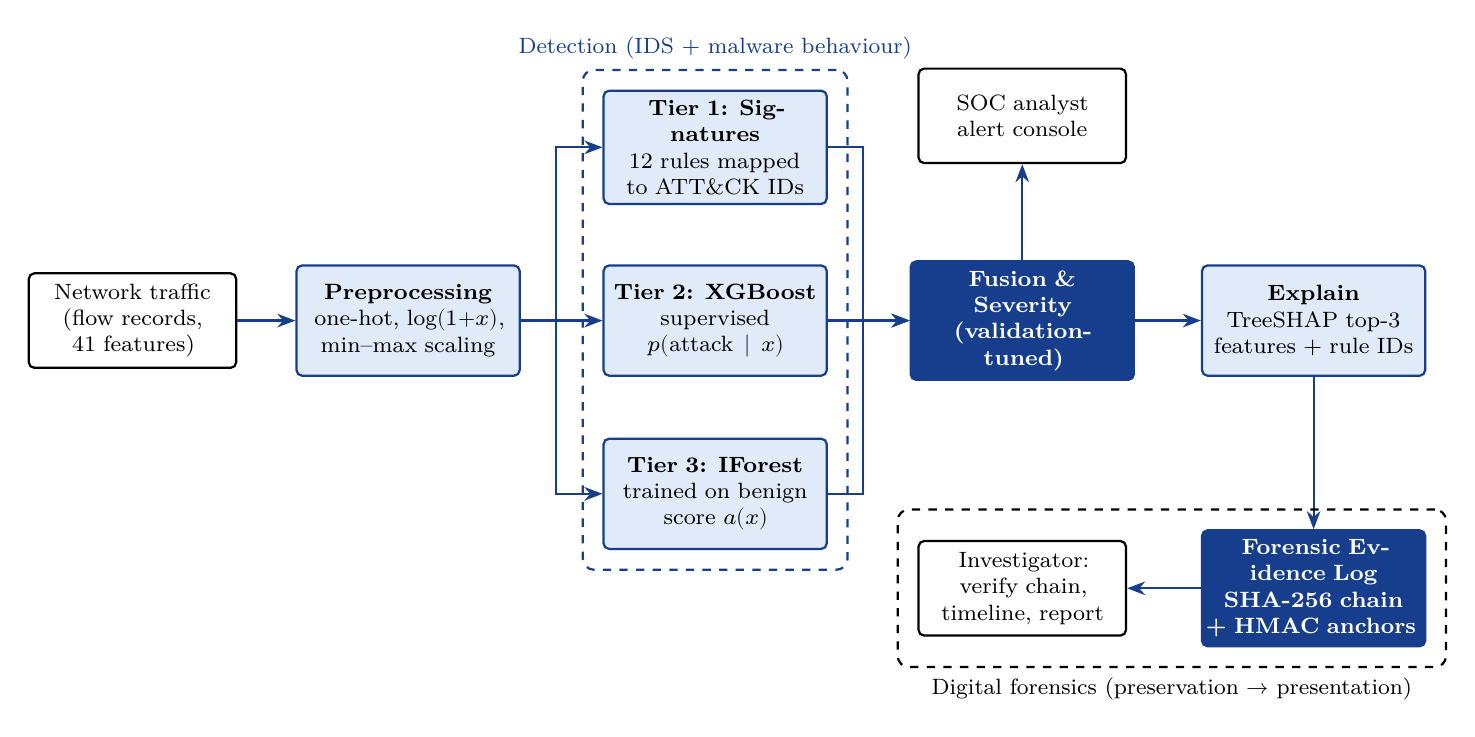
\begin{tikzpicture}[
  box/.style={draw=rblue,thick,rounded corners=2pt,fill=lblue,align=center,font=\footnotesize,minimum height=14mm,text width=26mm},
  dbox/.style={draw=rblue,thick,rounded corners=2pt,fill=rblue,text=white,align=center,font=\footnotesize\bfseries,minimum height=14mm,text width=26mm},
  wbox/.style={draw=black,thick,rounded corners=2pt,fill=white,align=center,font=\footnotesize,minimum height=12mm,text width=24mm},
  arr/.style={-{Stealth[length=2.3mm]},thick,rblue}]
\node[wbox] (in) at (0,0) {Network traffic\\(flow records,\\41 features)};
\node[box] (pre) at (3.5,0) {\textbf{Preprocessing}\\one-hot, $\log(1{+}x)$,\\min--max scaling};
\node[box] (t1) at (7.4,2.2) {\textbf{Tier 1: Signatures}\\12 rules mapped\\to ATT\&CK IDs};
\node[box] (t2) at (7.4,0) {\textbf{Tier 2: XGBoost}\\supervised\\$p(\text{attack}\mid x)$};
\node[box] (t3) at (7.4,-2.2) {\textbf{Tier 3: IForest}\\trained on benign\\score $a(x)$};
\node[dbox] (fus) at (11.3,0) {Fusion \&\\Severity\\(validation-tuned)};
\node[box] (shap) at (15.0,0) {\textbf{Explain}\\TreeSHAP top-3\\features + rule IDs};
\node[wbox] (soc) at (11.3,2.6) {SOC analyst\\alert console};
\node[dbox] (log) at (15.0,-3.4) {Forensic Evidence Log\\SHA-256 chain\\+ HMAC anchors};
\node[wbox] (ver) at (11.3,-3.4) {Investigator:\\verify chain,\\timeline, report};
\draw[arr] (in)--(pre);
\draw[arr] (pre.east)--++(0.45,0)|-(t1.west);
\draw[arr] (pre)--(t2);
\draw[arr] (pre.east)--++(0.45,0)|-(t3.west);
\draw[arr] (t1.east)--++(0.45,0)|-(fus.west);
\draw[arr] (t2)--(fus);
\draw[arr] (t3.east)--++(0.45,0)|-(fus.west);
\draw[arr] (fus)--(shap);
\draw[arr] (fus)--(soc);
\draw[arr] (shap)--(log);
\draw[arr] (log)--(ver);
\node[draw=rblue,dashed,thick,rounded corners,fit=(t1)(t2)(t3),inner sep=2.5mm,label={[font=\footnotesize\color{rblue}]above:Detection (IDS + malware behaviour)}] {};
\node[draw=black,dashed,thick,rounded corners,fit=(log)(ver),inner sep=2.5mm,label={[font=\footnotesize]below:Digital forensics (preservation $\rightarrow$ presentation)}] {};
\end{tikzpicture}}
\caption{Architecture of the proposed ForenSight framework.}\label{fig:arch}
\end{figure}

The methodology follows five phases that mirror the forensic process taught in Unit 4: \textbf{(1)} data acquisition and threat modelling; \textbf{(2)} preprocessing; \textbf{(3)} multi-tier detection and fusion; \textbf{(4)} explanation and evidence preservation; and \textbf{(5)} evaluation and verification.

\subsection{Phase 1: Dataset and Threat Model}\label{sec:data}
We use the NSL-KDD benchmark \cite{tavallaee2009detailed}. Each record summarises a network connection with 41 features in three groups: \emph{basic} features (duration, protocol, service, flag, bytes), \emph{content} features derived from payload inspection (failed logins, root shell, file creations), which are effectively host-level indicators similar to a HIDS, and \emph{traffic} features computed over 2-second and 100-connection windows (count, error rates, same-service rates). Attacks fall into four families, which we map to the threat model below.

\begin{itemize}
  \item \textbf{DoS} (Denial of Service), e.g.\ SYN flood (\texttt{neptune}), Smurf, Teardrop. ATT\&CK T1498/T1499.
  \item \textbf{Probe} (reconnaissance), e.g.\ \texttt{portsweep}, \texttt{nmap}, \texttt{satan}. ATT\&CK T1046/T1018.
  \item \textbf{R2L} (remote-to-local), e.g.\ \texttt{guess\_passwd} brute force and \texttt{warezmaster} illicit upload. Leaked dark-web credentials make these attacks cheaper. ATT\&CK T1110/T1105.
  \item \textbf{U2R} (user-to-root), e.g.\ \texttt{buffer\_overflow}, \texttt{rootkit}, \texttt{loadmodule}, i.e.\ malware-driven privilege escalation. ATT\&CK T1068.
\end{itemize}

\begin{table}[H]\centering\small
\caption{NSL-KDD composition used in this study. The test set contains 17 attack types never seen in training.}\label{tab:data}
\begin{tabular}{lrrrrrr}
\toprule
\textcolor{rblue}{Split} & \textcolor{rblue}{Normal} & \textcolor{rblue}{DoS} & \textcolor{rblue}{Probe} & \textcolor{rblue}{R2L} & \textcolor{rblue}{U2R} & \textcolor{rblue}{Total} \\ \midrule
KDDTrain+ & 67{,}343 & 45{,}927 & 11{,}656 & 995 & 52 & 125{,}973 \\
\quad training part (80\%, stratified) & \multicolumn{5}{c}{--} & 100{,}778 \\
\quad validation part (20\%, tuning only) & \multicolumn{5}{c}{--} & 25{,}195 \\
KDDTest+ & 9{,}711 & 7{,}460 & 2{,}421 & 2{,}885 & 67 & 22{,}544 \\
KDDTest-21 (hard subset) & \multicolumn{5}{c}{--} & 11{,}850 \\
\bottomrule
\end{tabular}

\vspace{3pt}{\footnotesize Attack types: 22 in training, 37 in test; \textbf{17 novel types with 3{,}750 records (29.2\% of test attacks)}. KDDTest-21 keeps records that most baseline classifiers misclassify.}
\end{table}

The 17 novel types (e.g.\ \texttt{apache2}, \texttt{mscan}, \texttt{processtable}, \texttt{snmpguess}, \texttt{httptunnel}, \texttt{sqlattack}, \texttt{xterm}, \texttt{worm}) act as a realistic stand-in for zero-day attacks. They allow us to measure Problem P1 directly, which a random train/test split would hide. Note also the class shift: R2L is 0.8\% of training data but 12.8\% of test data.

\subsection{Phase 2: Preprocessing}
\begin{enumerate}
  \item \textbf{Categorical encoding.} \texttt{protocol\_type} (3 values), \texttt{service} (70) and \texttt{flag} (11) are one-hot encoded. Encoders are fitted on training data only, and unseen categories map to all-zeros, giving \textbf{121 features}.
  \item \textbf{Heavy-tail compression.} Byte and count features span many orders of magnitude (e.g.\ \texttt{src\_bytes} up to $1.3\times10^{9}$). We therefore apply
  \begin{equation} x' = \ln(1+x) \end{equation}
  to twelve such features, which keeps magnitude ordering intact while preventing a few extreme flows from dominating.
  \item \textbf{Scaling.} Numeric features are min--max normalised using training statistics, $\tilde{x} = (x' - \min_{\text{train}})/(\max_{\text{train}}-\min_{\text{train}})$.
  \item \textbf{Leakage-free split.} KDDTrain+ is split 80/20 with stratification by attack label. The \emph{validation} part is the only data used for threshold selection. KDDTest+ is touched exactly once, for final reporting, which avoids the data-snooping pitfall identified by Arp \emph{et al.}\ \cite{arp2022dos}.
\end{enumerate}

\subsection{Phase 3a: Tier 1 --- Signature Engine}
Following Snort's design philosophy \cite{roesch1999snort}, we wrote 12 transparent rules from attack and malware behaviour described in the literature \cite{sikorski2012practical,scarfone2007sp80094}. Each rule has an ID, a human-readable name and an ATT\&CK technique, so an alert is self-documenting for the forensic report. Table~\ref{tab:rules} lists the rules together with their measured hit counts and precision on KDDTest+.

\begin{table}[H]\centering\small
\caption{Signature rules (Tier 1), ATT\&CK mapping and measured performance on KDDTest+.}\label{tab:rules}
\begin{tabularx}{\linewidth}{l Y p{4.4cm} c r r}
\toprule
\textcolor{rblue}{ID} & \textcolor{rblue}{Behaviour detected} & \textcolor{rblue}{Condition (simplified)} & \textcolor{rblue}{ATT\&CK} & \textcolor{rblue}{Hits} & \textcolor{rblue}{Prec.} \\ \midrule
SIG-01 & SYN flood (half-open) & flag$\in\{$S0..S3$\}$, serror\_rate$\geq$0.8, count$\geq$50 & T1498/9 & 1{,}492 & 1.000 \\
SIG-02 & ICMP Smurf flood & icmp, ecr\_i, src\_bytes$\geq$1000 & T1498 & 594 & 0.950 \\
SIG-03 & Malformed fragments & wrong\_fragment$>$0 & T1499 & 100 & 0.480 \\
SIG-04 & LAND attack & land$=$1 & T1499 & 7 & 1.000 \\
SIG-05 & Port scan / sweep & rerror\_rate$\geq$0.8 \& diff\_srv$\geq$0.5 & T1046 & 1{,}201 & 0.955 \\
SIG-06 & ICMP host sweep & icmp echo, srv\_diff\_host$\geq$0.5 & T1018 & 177 & 0.932 \\
SIG-07 & Brute-force login & num\_failed\_logins$\geq$1 & T1110 & 478 & 0.990 \\
SIG-08 & Root shell obtained & root\_shell$\geq$1 & T1068 & 55 & 0.673 \\
SIG-09 & su / root activity & su\_attempted, or root ops + file creation & T1548 & 26 & 0.846 \\
SIG-10 & Oversized HTTP request & http, src\_bytes$\geq$20{,}000 & T1190 & 816 & 0.993 \\
SIG-11 & Guest FTP write (warez) & ftp/ftp\_data, guest login & T1105 & 639 & 0.931 \\
SIG-12 & Many ``hot'' indicators & hot$\geq$5 & T1059 & 39 & 0.282 \\
\bottomrule
\end{tabularx}
\end{table}

\subsection{Phase 3b: Tier 2 --- Supervised Classifiers}
Five classifiers representing different inductive biases were trained on the same features (Table~\ref{tab:hyper}). XGBoost was selected as the Tier-2 engine because it had the highest validation accuracy and ROC-AUC (Section~\ref{sec:results}). It fits an additive ensemble of $K$ regression trees $f_k$ by minimising a regularised objective \cite{chen2016xgboost}:
\begin{equation}
\mathcal{L} = \sum_{i=1}^{n} \ell\big(y_i,\hat{y}_i\big) + \sum_{k=1}^{K}\Omega(f_k),\qquad \Omega(f)=\gamma T+\tfrac{1}{2}\lambda\lVert w\rVert^{2},
\end{equation}
where $\ell$ is the logistic loss, $T$ the number of leaves and $w$ the leaf weights. The regularisation term $\Omega$ penalises complex trees, which matters when the test distribution shifts.

\begin{table}[H]\centering\small
\caption{Models and hyper-parameters (all with random seed 42).}\label{tab:hyper}
\begin{tabularx}{\linewidth}{l Y Y}
\toprule
\textcolor{rblue}{Model} & \textcolor{rblue}{Key hyper-parameters} & \textcolor{rblue}{Rationale} \\ \midrule
Logistic Regression & L2, $C=1.0$, max\_iter 2000 & Linear baseline \\
Decision Tree & max\_depth 20, min\_samples\_leaf 2 & Interpretable rules \\
Random Forest \cite{breiman2001random} & 200 trees, bootstrap & Variance reduction via bagging \\
MLP & (64, 32) ReLU, Adam, early stopping & Non-linear neural baseline \\
\textbf{XGBoost} \cite{chen2016xgboost} & 300 trees, depth 8, $\eta=0.1$, subsample 0.9, colsample 0.8 & Boosting, regularised, fast TreeSHAP \\
Isolation Forest \cite{liu2008isolation} & 300 trees, 4{,}096 samples/tree, \textbf{benign data only} & Label-free novelty detection \\
\bottomrule
\end{tabularx}
\end{table}

\subsection{Phase 3c: Tier 3 --- Anomaly Detector for Zero-Day Attacks}
Isolation Forest is trained \emph{only on benign training flows}, so it models ``normal'' and flags anything easy to isolate. For a point $x$ with average path length $E[h(x)]$ over the trees, the anomaly score is
\begin{equation}
a(x) = 2^{-\frac{E[h(x)]}{c(\psi)}},\qquad c(\psi)=2H(\psi-1)-\frac{2(\psi-1)}{\psi},
\end{equation}
where $\psi$ is the sub-sample size and $H$ the harmonic number \cite{liu2008isolation}. Its threshold is \emph{calibrated} rather than guessed: $\tau_a = Q_q\big(\{a(x): x\in V_{\text{benign}}\}\big)$, the $q$-quantile of scores on validation benign traffic. This fixes the expected false-alarm rate of the tier at about $1-q$.

\subsection{Phase 3d: Fusion and Threshold Optimisation}\label{sec:fusion}
The tiers are combined with a logical OR, so each covers the others' blind spots:
\begin{equation}
\hat{y}(x) = \mathbb{1}\big[S(x)\big] \;\lor\; \mathbb{1}\big[p(x)\ge\tau_m\big] \;\lor\; \mathbb{1}\big[a(x)\ge\tau_a\big],
\end{equation}
where $S(x)$ is true if any signature fires and $p(x)$ is the XGBoost attack probability. Because OR-fusion raises recall at the cost of false positives, the two thresholds are chosen by a \textbf{constrained grid search on validation data only}:
\begin{equation}
(\tau_m^{*},q^{*}) = \arg\max_{\tau_m\in\{0.05,\dots,0.95\},\;q\in\{0.90,\dots,0.99\}} F_1^{V}(\tau_m,q)\quad\text{s.t.}\quad \mathrm{FPR}^{V}(\tau_m,q)\le 3\%.
\end{equation}
The 3\% budget reflects an analyst's practical alert-handling capacity. The search selected $\tau_m^{*}=0.45$ and $q^{*}=0.99$. Severity is \textsc{High} if a signature fires or $p(x)\ge0.9$, \textsc{Medium} if $p(x)\ge\tau_m$, and \textsc{Low} for anomaly-only alerts, which tells analysts what to triage first. Algorithm~\ref{alg:detect} summarises the per-flow procedure.

\begin{algorithm}[H]
\caption{ForenSight per-flow detection and evidence logging}\label{alg:detect}
\KwIn{flow record $r$; rules $\mathcal{R}$; XGBoost $f$; IForest $g$; thresholds $\tau_m,\tau_a$; last hash $H_{\text{prev}}$; anchor key $K$}
\KwOut{alert decision, evidence record $E$}
$x \leftarrow \textsc{Preprocess}(r)$\;
$\mathit{hits}\leftarrow\{\rho.\mathit{id} : \rho\in\mathcal{R},\ \rho(r)=\text{true}\}$ \tcp*{Tier 1}
$p \leftarrow f(x)$;\quad $a\leftarrow g(x)$ \tcp*{Tiers 2 and 3}
\If{$\mathit{hits}\neq\emptyset \lor p\ge\tau_m \lor a\ge\tau_a$}{
  $\mathit{sev}\leftarrow$ \textsc{High} if $\mathit{hits}\neq\emptyset\lor p\ge 0.9$; else \textsc{Medium} if $p\ge\tau_m$; else \textsc{Low}\;
  $\phi\leftarrow \textsc{TreeSHAP}(f,x)$;\quad $\mathit{ev}\leftarrow$ top-3 features by $|\phi_j|$ \tcp*{explain}
  $E\leftarrow\{\mathit{seq},\mathit{ts},\mathit{flow},\mathit{hits},p,a,\mathit{sev},\mathit{ev},\mathit{prev\_hash}{=}H_{\text{prev}}\}$\;
  $E.\mathit{hash}\leftarrow \mathrm{SHA256}(\textsc{Canonical}(E))$;\quad $H_{\text{prev}}\leftarrow E.\mathit{hash}$ \tcp*{preserve}
  \lIf{$(\mathit{seq}+1)\bmod 1000=0$}{publish anchor $\langle \mathit{seq}, H_{\text{prev}}, \mathrm{HMAC}_K(H_{\text{prev}})\rangle$ to WORM store}
  \Return \textsc{Alert}, $E$\;
}
\Return \textsc{Benign}\;
\end{algorithm}

\subsection{Phase 4a: Explainability with SHAP}
For each alert, TreeSHAP decomposes the model output into additive feature contributions \cite{lundberg2017unified,lundberg2020local}:
\begin{equation}
f(x)=\phi_0+\sum_{j=1}^{M}\phi_j,\qquad
\phi_j=\sum_{S\subseteq F\setminus\{j\}}\frac{|S|!\,(M-|S|-1)!}{M!}\Big[f_{S\cup\{j\}}(x)-f_S(x)\Big].
\end{equation}
The three features with the largest $|\phi_j|$ are stored in the evidence record. This gives investigators a specific, testable reason for each alert, for example ``\texttt{src\_bytes}, \texttt{count} and \texttt{service\_private} pushed this flow towards \emph{attack}''.

\subsection{Phase 4b: Forensic Evidence Preservation}\label{sec:forensic}
\paragraph{Hash chain.} Each alert record $R_i$ (canonical JSON with sorted keys) embeds the hash of its predecessor:
\begin{equation}
H_0 = 0^{256},\qquad H_i=\mathrm{SHA256}\big(\textsc{Canonical}(R_i \,\|\, H_{i-1})\big).
\end{equation}
Changing, deleting or re-ordering any record changes every later hash. This is the hash-linking principle of Haber and Stornetta \cite{haber1991time}, applied to IDS alerts.

\paragraph{Keyed anchors.} A hash chain alone does not stop an attacker who rewrites a record and \emph{recomputes all later hashes}. Every 1{,}000 alerts we therefore publish an anchor $A_k=\langle k, H_k, \mathrm{HMAC}_K(H_k)\rangle$ to write-once storage, with key $K$ kept outside the monitored host (e.g.\ in an HSM). An attacker without $K$ cannot forge anchors, so a fully re-hashed chain is still detected. This follows the forward-integrity idea of Schneier and Kelsey \cite{schneier1999secure}.

\begin{figure}[H]\centering
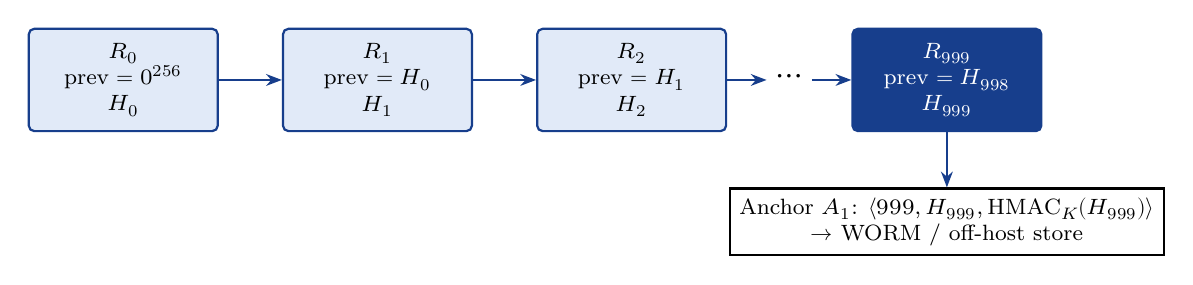
\begin{tikzpicture}[rec/.style={draw=rblue,thick,fill=lblue,rounded corners=2pt,minimum width=24mm,minimum height=13mm,align=center,font=\footnotesize},
  arr/.style={-{Stealth[length=2mm]},thick,rblue}]
\node[rec] (r0) {$R_0$\\ prev $=0^{256}$\\ $H_0$};
\node[rec,right=8mm of r0] (r1) {$R_1$\\ prev $=H_0$\\ $H_1$};
\node[rec,right=8mm of r1] (r2) {$R_2$\\ prev $=H_1$\\ $H_2$};
\node[right=5mm of r2,font=\large] (dots) {$\cdots$};
\node[rec,right=5mm of dots,fill=rblue,text=white] (r999) {$R_{999}$\\ prev $=H_{998}$\\ $H_{999}$};
\node[draw=black,thick,below=7mm of r999,align=center,font=\footnotesize,fill=white] (anc) {Anchor $A_1$: $\langle 999, H_{999}, \mathrm{HMAC}_K(H_{999})\rangle$\\$\rightarrow$ WORM / off-host store};
\draw[arr] (r0)--(r1); \draw[arr] (r1)--(r2); \draw[arr] (r2)--(dots); \draw[arr] (dots)--(r999); \draw[arr] (r999)--(anc);
\end{tikzpicture}
\caption{Tamper-evident evidence log: SHA-256 hash chain sealed by periodic HMAC anchors.}\label{fig:chain}
\end{figure}

\paragraph{Verification.} Algorithm~\ref{alg:verify} is run by the investigator, independently of the IDS host. It reports both \emph{whether} the log was tampered with and \emph{where}.

\begin{algorithm}[H]
\caption{Evidence-log verification}\label{alg:verify}
\KwIn{log $L=[E_0,\dots,E_{n-1}]$; anchors $\mathcal{A}$; key $K$}
$h\leftarrow 0^{256}$\;
\For{$i\leftarrow 0$ \KwTo $n-1$}{
  \lIf{$E_i.\mathit{prev\_hash}\neq h$ \textbf{or} $E_i.\mathit{seq}\neq i$}{\Return (\textsc{BrokenLink}, $i$)}
  \lIf{$\mathrm{SHA256}(\textsc{Canonical}(E_i\setminus\mathit{hash}))\neq E_i.\mathit{hash}$}{\Return (\textsc{HashMismatch}, $i$)}
  $h\leftarrow E_i.\mathit{hash}$\;
}
\ForEach{$\langle k,H_k,\sigma\rangle\in\mathcal{A}$}{
  \lIf{$k\ge n$ \textbf{or} $E_k.\mathit{hash}\neq H_k$ \textbf{or} $\sigma\neq\mathrm{HMAC}_K(H_k)$}{\Return (\textsc{AnchorMismatch}, $k$)}
}
\Return \textsc{Intact}\;
\end{algorithm}

Table~\ref{tab:nist} shows how this design satisfies each phase of the digital-forensics process from Unit 4 and NIST SP 800-86 \cite{kent2006sp80086}.

\begin{table}[H]\centering\small
\caption{Alignment of ForenSight with the digital-forensics process.}\label{tab:nist}
\begin{tabularx}{\linewidth}{>{\bfseries}p{3.0cm} Y}
\toprule
\textcolor{rblue}{Forensic phase} & \textcolor{rblue}{ForenSight mechanism} \\ \midrule
Identification & Three-tier detection identifies which flows are potential evidence; severity ranks them \\
Preservation & SHA-256 hash chain + HMAC anchors in write-once storage; canonical JSON prevents ambiguity \\
Collection & Each record stores flow ID, timestamp, protocol/service/flag, byte counts and detector outputs \\
Analysis & Rule IDs, ATT\&CK techniques, ML probability, anomaly score, SHAP top-3 features; timeline from sequence numbers \\
Documentation & Self-describing JSON records; verification output gives position of any tampering \\
Presentation & Verifiable integrity proof supports the certificate requirement for electronic records under BSA 2023 \S63 \cite{bsa2023} \\
\bottomrule
\end{tabularx}
\end{table}

\subsection{Phase 5: Evaluation Metrics and Protocol}
With TP, FP, TN and FN counted with \emph{attack} as the positive class:
\begin{gather}
\text{Accuracy}=\frac{TP+TN}{TP+TN+FP+FN},\qquad \text{Precision}=\frac{TP}{TP+FP},\\
\text{Recall (DR)}=\frac{TP}{TP+FN},\qquad F_1=\frac{2\cdot\text{Precision}\cdot\text{Recall}}{\text{Precision}+\text{Recall}},\\
\text{FPR}=\frac{FP}{FP+TN}.
\end{gather}
We also report ROC-AUC, \emph{novel-attack recall} (recall restricted to the 17 unseen types), per-family recall, inference latency per flow, and for the evidence log, the \emph{tamper-detection rate} over 200 randomised trials for each of five attack classes on a 2{,}000-alert log.

\subsection{Justification of Design Choices}
\begin{table}[H]\centering\small
\caption{Key design decisions, alternatives considered and justification.}\label{tab:just}
\begin{tabularx}{\linewidth}{p{3.2cm} p{3.4cm} Y}
\toprule
\textcolor{rblue}{Decision} & \textcolor{rblue}{Alternative} & \textcolor{rblue}{Justification} \\ \midrule
Hybrid three-tier IDS & Single ML model & Single models fail on unseen attacks (closed-world problem \cite{sommer2010outside}); our ablation confirms this (Table~\ref{tab:abl}) \\
XGBoost as Tier 2 & Deep neural network & Highest validation accuracy/AUC on tabular data; fast exact TreeSHAP; small CPU footprint \\
Isolation Forest as Tier 3 & One-class SVM, autoencoder & Linear time, needs no attack labels, few hyper-parameters, robust with a calibrated threshold \\
OR-fusion with FPR budget & Weighted voting / stacking & Keeps each tier's high-precision alerts; the constraint keeps false alarms manageable for analysts \\
Validation-only tuning & Tuning on test set & Avoids data snooping \cite{arp2022dos}; reported test scores are honest estimates \\
Hash chain + HMAC anchors & Plain logs / blockchain & Detects edits, deletions and re-ordering at microsecond cost; anchors defeat re-hashing; no consensus overhead \\
NSL-KDD benchmark & Random split of one dataset & Built-in novel attack types allow a direct zero-day evaluation; enables comparison with prior work \\
\bottomrule
\end{tabularx}
\end{table}

% ============================ 4. IMPLEMENTATION ============================
\section{Implementation Details}
\subsection{Environment and Tools}
\begin{table}[H]\centering\small
\caption{Implementation environment.}\label{tab:env}
\begin{tabular}{ll}
\toprule
\textcolor{rblue}{Component} & \textcolor{rblue}{Version / Specification} \\ \midrule
Hardware & Intel Xeon @ 2.80\,GHz, 2 vCPU, 8\,GB RAM (no GPU) \\
Language & Python 3.13 \\
ML libraries & scikit-learn 1.9.1 \cite{pedregosa2011scikit}, XGBoost 3.4.1 \cite{chen2016xgboost}, SHAP 0.52.0 \cite{lundberg2017unified} \\
Data handling & pandas 3.0.5, NumPy 2.5.3 \\
Cryptography & Python \texttt{hashlib} (SHA-256), \texttt{hmac} (HMAC-SHA256) \\
Visualisation & Matplotlib \\
Dataset & NSL-KDD \texttt{KDDTrain+.txt}, \texttt{KDDTest+.txt} \cite{tavallaee2009detailed} \\
Reproducibility & Fixed random seed 42 for split, models and tamper trials \\
\bottomrule
\end{tabular}
\end{table}

\subsection{Software Modules}
The implementation (\(\approx\)300 lines of Python) is organised into seven modules that correspond to the methodology phases:
\begin{enumerate}
  \item \texttt{load\_data}: reads NSL-KDD, maps 39 attack labels to the four families, and flags the 17 novel types.
  \item \texttt{preprocess}: \texttt{ColumnTransformer} with one-hot encoding and min--max scaling after $\log(1{+}x)$.
  \item \texttt{signature\_engine}: the 12 rules as vectorised boolean predicates over flow features.
  \item \texttt{train\_models}: trains the five classifiers and the Isolation Forest, and records fit time and latency.
  \item \texttt{fusion}: validation grid search under the FPR constraint, severity assignment and ablation.
  \item \texttt{explain}: TreeSHAP for global importance and per-alert top-3 evidence.
  \item \texttt{evidence\_log}: hash chaining, HMAC anchors, verification and the tamper-simulation harness.
\end{enumerate}

\subsection{Key Code Excerpts}
\noindent\textbf{Signature rules as data.} Each rule is a tuple (ID, description, ATT\&CK ID, predicate), so new threat intelligence (for example indicators from dark-web monitoring) can be added without changing the engine:
\begin{lstlisting}[language=Python]
RULES = [
 ("SIG-01", "SYN flood (half-open connections)", "T1498/T1499",
  lambda d: d.flag.isin(["S0","S1","S2","S3"]) & (d.serror_rate >= 0.8) & (d["count"] >= 50)),
 ("SIG-07", "Brute-force login (failed logins)", "T1110",
  lambda d: d.num_failed_logins >= 1),
 ("SIG-08", "Root shell obtained (privilege escalation)", "T1068",
  lambda d: d.root_shell >= 1),
 # ... 9 more rules
]
hits = np.column_stack([f(df).values for (_, _, _, f) in RULES])   # vectorised
\end{lstlisting}

\noindent\textbf{Hash-chained evidence record.} Canonical serialisation (sorted keys, no whitespace) ensures the verifier recomputes exactly the same bytes:
\begin{lstlisting}[language=Python]
rec = {"seq": k, "ts": ts, "flow_id": i, "detector": src, "rules": rule_ids,
       "ml_score": p, "anomaly": a, "severity": sev,
       "evidence": top3_shap_features, "prev_hash": prev}
payload = json.dumps(rec, sort_keys=True, separators=(",", ":")).encode()
rec["hash"] = hashlib.sha256(payload).hexdigest();  prev = rec["hash"]
if (k + 1) % 1000 == 0:                      # keyed anchor -> WORM store
    anchors.append({"upto": k, "hash": prev,
                    "hmac": hmac.new(KEY, prev.encode(), hashlib.sha256).hexdigest()})
\end{lstlisting}

\noindent\textbf{A real evidence record} produced by the system (the first alert in the KDDTest+ run):
\begin{lstlisting}[numbers=none,basicstyle=\ttfamily\footnotesize]
{"seq": 0, "ts": 1791436800.0, "flow_id": 0, "proto": "tcp", "service": "private",
 "flag": "REJ", "src_bytes": 0, "dst_bytes": 0, "detector": "ML", "rules": [],
 "ml_score": 1.0, "anomaly": 0.5669, "severity": "HIGH",
 "evidence": ["src_bytes", "count", "service_private"],
 "prev_hash": "0000000000000000000000000000000000000000000000000000000000000000",
 "hash": "05c1f94a925086a6e9bf2b196911de4f9b74084f78b19152b50624586395698c"}
\end{lstlisting}

\subsection{Tamper-Simulation Harness}
To test the evidence log the way an intruder would attack it, the harness copies a 2{,}000-alert log 200 times for each of five manipulations, applies one random manipulation per copy, and runs Algorithm~\ref{alg:verify}:
\begin{enumerate*}[label=(\roman*)]
  \item \emph{field modification}: change an alert's detector to ``NONE'' and severity to ``LOW'';
  \item \emph{record deletion}, with the attacker re-numbering later sequence numbers;
  \item \emph{re-ordering} of two adjacent records;
  \item \emph{modify and fully re-hash} every later record (an attacker who understands the chain but lacks $K$);
  \item \emph{tail truncation} (deleting the most recent alerts).
\end{enumerate*}

% ============================ 5. RESULTS ============================
\section{Results and Discussion}\label{sec:results}
\subsection{Binary Detection Performance}
Table~\ref{tab:main} compares all detectors on KDDTest+ and the hard KDDTest-21 subset. The final column shows validation accuracy, to make the generalisation gap visible.

\begin{table}[H]\centering\small
\caption{Binary detection results (attack = positive). Best value per column in \textbf{bold}.}\label{tab:main}
\setlength{\tabcolsep}{4.2pt}
\resizebox{\linewidth}{!}{%
\begin{tabular}{l cccccc cc c}
\toprule
& \multicolumn{6}{c}{\textcolor{rblue}{KDDTest+ (22{,}544 flows)}} & \multicolumn{2}{c}{\textcolor{rblue}{KDDTest-21}} & \textcolor{rblue}{Val.}\\
\cmidrule(lr){2-7}\cmidrule(lr){8-9}\cmidrule(lr){10-10}
\textcolor{rblue}{Detector} & Acc. & Prec. & Recall & F1 & FPR & AUC & Acc. & F1 & Acc. \\ \midrule
Signature engine (Tier 1) & 65.18 & 96.30 & 40.38 & 0.569 & 2.05 & -- & 52.42 & 0.601 & 86.35 \\
Logistic Regression & 74.56 & 91.27 & 61.15 & 0.732 & 7.73 & 0.776 & 51.73 & 0.622 & 98.29 \\
Decision Tree & 78.94 & 91.30 & 69.63 & 0.790 & 8.76 & 0.827 & 60.33 & 0.712 & 99.80 \\
Random Forest & 78.72 & \textbf{96.98} & 64.62 & 0.776 & 2.66 & 0.959 & 59.51 & 0.683 & 99.87 \\
MLP (64-32) & 79.60 & 92.69 & 69.66 & 0.795 & 7.26 & 0.903 & 61.21 & 0.716 & 99.73 \\
XGBoost (Tier 2) & 79.20 & 96.87 & 65.58 & 0.782 & 2.80 & \textbf{0.966} & 60.44 & 0.693 & \textbf{99.92} \\
Isolation Forest (Tier 3)$^\dagger$ & 82.35 & 96.86 & 71.32 & 0.822 & 3.06 & 0.956 & 66.48 & 0.752 & -- \\ \midrule
\textbf{ForenSight hybrid} & \textbf{87.23} & 96.48 & \textbf{80.50} & \textbf{0.878} & 3.88 & 0.957 & \textbf{75.86} & \textbf{0.834} & 98.61 \\
\bottomrule
\multicolumn{10}{l}{\footnotesize $^\dagger$Stand-alone IForest uses a 3\% validation FPR budget ($q{=}0.97$); inside the hybrid it uses $q^{*}{=}0.99$. Acc., Prec., Recall, FPR in \%.}
\end{tabular}}
\end{table}

\begin{keybox}{Key Findings}
\begin{itemize}[leftmargin=12pt]
\item \textbf{Hybrid wins clearly:} +8.0 points accuracy and +14.9 points recall over XGBoost on KDDTest+, and +15.4 points accuracy on KDDTest-21, with precision kept above 96\%.
\item \textbf{Large generalisation gap for single models:} XGBoost scores 99.92\% on validation but only 79.20\% on the test set. This is the closed-world problem \cite{sommer2010outside} measured directly.
\item \textbf{Cost:} false-positive rate rises modestly from 2.80\% to 3.88\%, i.e.\ about 105 extra false alarms among 9{,}711 benign flows.
\end{itemize}
\end{keybox}

For context, Tavallaee \emph{et al.}\ reported a best accuracy of about 82\% on KDDTest+ and 66\% on KDDTest-21 among seven classical classifiers \cite{tavallaee2009detailed}. Our single classifiers (79--80\% and 60--61\%) are consistent with that range, which supports the validity of our setup. The hybrid exceeds both figures.

Figure~\ref{fig:roc} shows ROC curves. XGBoost has the highest AUC (0.966) and Logistic Regression the lowest (0.776), which confirms that the attack boundary is strongly non-linear. AUC measures ranking ability over all thresholds, but an IDS operates at \emph{one} threshold. The hybrid's fused score has a slightly lower AUC (0.957), yet it gives the best F1 at the chosen operating point because it combines three \emph{different kinds} of evidence.

\begin{figure}[H]\centering
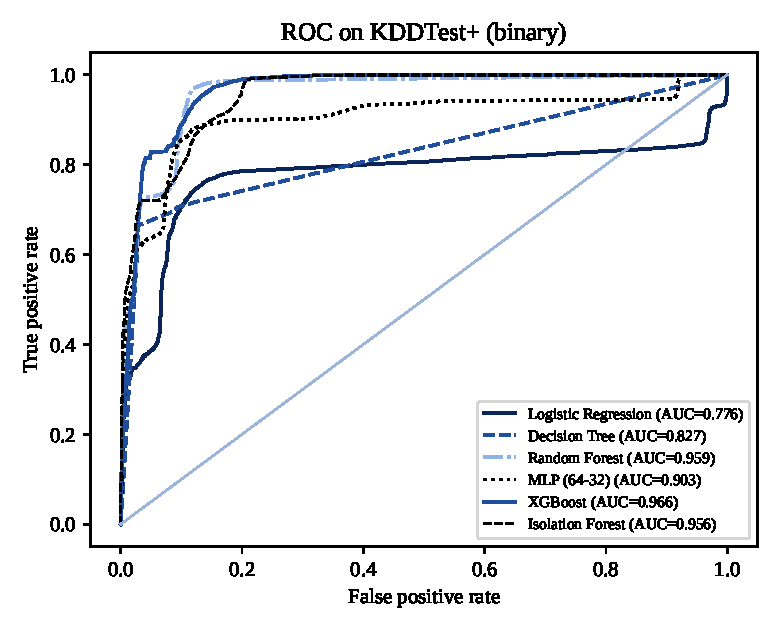
\includegraphics[width=0.66\linewidth]{figures/roc.pdf}
\caption{ROC curves on KDDTest+ for all learned detectors.}\label{fig:roc}
\end{figure}

\subsection{Ablation Study: What Does Each Tier Contribute?}
\begin{table}[H]\centering\small
\caption{Ablation on KDDTest+ (thresholds from validation tuning). Values in \%, F1 as a fraction.}\label{tab:abl}
\begin{tabular}{lccccc}
\toprule
\textcolor{rblue}{Configuration} & \textcolor{rblue}{Accuracy} & \textcolor{rblue}{Recall} & \textcolor{rblue}{Novel-attack recall} & \textcolor{rblue}{FPR} & \textcolor{rblue}{F1} \\ \midrule
Signature only & 65.18 & 40.38 & 31.47 & 2.05 & 0.569 \\
XGBoost only ($t{=}0.5$) & 79.20 & 65.58 & 37.04 & 2.80 & 0.782 \\
XGBoost (tuned $t{=}0.45$) & 79.32 & 65.81 & 37.68 & 2.82 & 0.784 \\
Isolation Forest only ($q{=}0.99$) & 76.53 & 60.24 & 53.92 & 1.96 & 0.745 \\
Signature + XGBoost & 84.54 & 75.61 & 45.52 & 3.66 & 0.848 \\
XGBoost + Isolation Forest & 83.45 & 73.27 & 61.76 & 3.11 & 0.834 \\
\textbf{Full hybrid (Sig + XGB + IF)} & \textbf{87.23} & \textbf{80.50} & \textbf{62.16} & 3.88 & \textbf{0.878} \\
\bottomrule
\end{tabular}
\end{table}

\begin{figure}[H]\centering
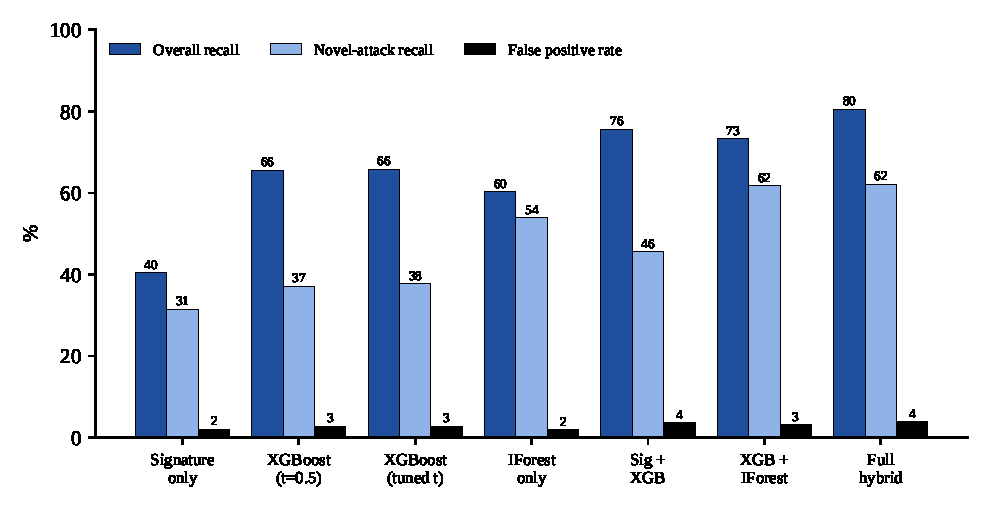
\includegraphics[width=0.86\linewidth]{figures/ablation.pdf}
\caption{Ablation: overall recall, novel-attack recall and false-positive rate per configuration.}\label{fig:abl}
\end{figure}

The ablation (Table~\ref{tab:abl}, Figure~\ref{fig:abl}) shows that \textbf{each tier contributes something the others do not}:
\begin{itemize}
  \item \textbf{Signatures add 10 points of recall to XGBoost} (65.6\% $\rightarrow$ 75.6\%). Most of this gain is in R2L brute force and warez attacks, whose decisive evidence is a single content feature (\texttt{num\_failed\_logins}, guest FTP login) that the ML model under-weights because R2L is only 0.8\% of training data.
  \item \textbf{The anomaly tier is the zero-day specialist.} On its own it has the best novel-attack recall (53.9\% vs.\ 37.0\% for XGBoost), and adding it to XGBoost raises novel recall to 61.8\%. It is the only tier that does not depend on prior knowledge of attacks.
  \item \textbf{Tier attribution:} of the 10{,}331 attacks the hybrid detected, 5{,}182 were caught by signatures, 4{,}521 only by XGBoost and 628 only by the anomaly detector. 2{,}502 attacks (19.5\%) were missed.
\end{itemize}

\subsection{Detection by Attack Family and Novelty}
\begin{figure}[H]\centering
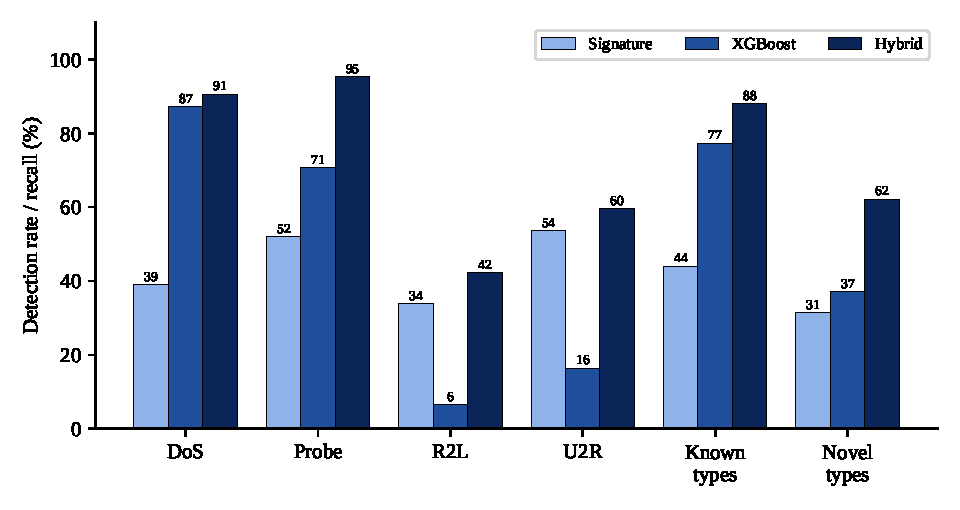
\includegraphics[width=0.88\linewidth]{figures/cat_recall.pdf}
\caption{Detection rate per attack family and for known vs.\ novel attack types on KDDTest+.}\label{fig:cat}
\end{figure}

Figure~\ref{fig:cat} shows that DoS (91\%) and Probe (95\%) attacks are detected reliably, because they create strong volumetric patterns (high \texttt{count}, error rates). \textbf{R2L} (42\%) and \textbf{U2R} (60\%) are much harder. XGBoost alone detects only 6\% of R2L and 16\% of U2R. Signatures help here (34\% and 54\%), because these attacks show up in host-level content features rather than traffic volume, which is the same reason Unit 4 distinguishes NIDS from HIDS. For the 17 novel types, recall rises from 37\% (XGBoost) to 62\% (hybrid).

\paragraph{Attack-level error analysis.} Looking at individual attack types explains the remaining misses:
\begin{itemize}
  \item \texttt{mscan} (novel probe, 996 flows): XGBoost 29\% $\rightarrow$ hybrid \textbf{89\%}, mainly due to the anomaly tier and SIG-05.
  \item \texttt{apache2} (novel DoS, 737 flows): hybrid \textbf{98\%}; SIG-10 (oversized HTTP) alone catches 79\%.
  \item \texttt{httptunnel} (novel R2L, 133 flows): signatures and XGBoost catch under 1\%; the anomaly tier lifts the hybrid to 56\%.
  \item \texttt{guess\_passwd} (1{,}231 flows): XGBoost detects \textbf{0\%}, because the training set has only 53 examples; SIG-07 detects 38\%. The remaining flows were single connections with no recorded failed login.
  \item \texttt{snmpgetattack} / \texttt{snmpguess} (509 flows): \textbf{0\%} for every detector. We checked the data: 72 of these 509 records are feature-for-feature identical to benign records in NSL-KDD, and the rest look like ordinary SNMP polling at the flow level, so no flow-level detector can separate them. Payload inspection (the SNMP community string) would be required, which we note as a data limitation rather than a modelling one.
\end{itemize}

\subsection{Multi-Class Attack Attribution}
For forensic reporting, knowing \emph{which kind} of attack occurred matters as much as detecting it. A class-balanced 5-class XGBoost reached 78.3\% accuracy, weighted-F1 0.745 and macro-F1 0.590 (per-class F1: Normal 0.806, DoS 0.898, Probe 0.756, R2L 0.147, U2R 0.341). The confusion matrix (Figure~\ref{fig:cm}) shows that the dominant error is R2L predicted as Normal (2{,}641 of 2{,}885 flows), which matches the binary analysis above.

\begin{figure}[H]\centering
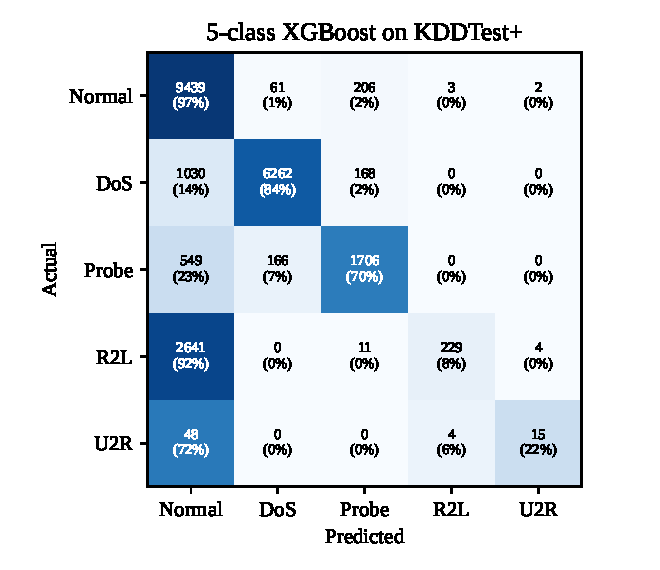
\includegraphics[width=0.56\linewidth]{figures/cm5.pdf}
\caption{Confusion matrix of the 5-class XGBoost on KDDTest+ (counts and row-normalised \%).}\label{fig:cm}
\end{figure}

\subsection{Explainability Results}
\begin{figure}[H]\centering
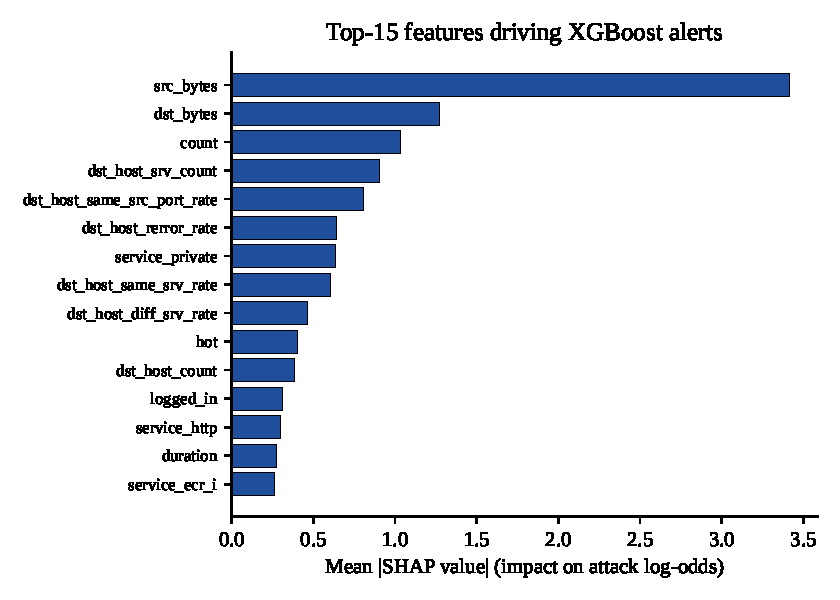
\includegraphics[width=0.74\linewidth]{figures/shap.pdf}
\caption{Global SHAP importance (mean $|\phi_j|$ over 3{,}000 test flows) for the Tier-2 XGBoost model.}\label{fig:shap}
\end{figure}

Figure~\ref{fig:shap} shows that \texttt{src\_bytes} is by far the most influential feature (mean $|\phi|=3.42$), followed by \texttt{dst\_bytes}, \texttt{count} and \texttt{dst\_host\_srv\_count}. These are the same indicators a human analyst uses: payload size separates floods and exploits from normal sessions, and connection counts expose scans and DoS. Because the model's reasoning matches domain knowledge, analysts and courts have more reason to trust it, and the absence of content features such as \texttt{num\_failed\_logins} from the top 15 confirms \emph{why} XGBoost misses R2L attacks and why the signature tier is needed.

\subsection{Forensic Evidence Log: Integrity and Overhead}
\begin{table}[H]\centering\small
\caption{Tamper-detection results (200 randomised trials per manipulation on a 2{,}000-alert log).}\label{tab:tamper}
\resizebox{\linewidth}{!}{%
\begin{tabular}{lccc}
\toprule
\textcolor{rblue}{Manipulation by attacker} & \textcolor{rblue}{Detected} & \textcolor{rblue}{Exact location found} & \textcolor{rblue}{Detection mechanism} \\ \midrule
Field modification & 200/200 & 200/200 & Hash mismatch \\
Record deletion (+ re-numbering) & 200/200 & 200/200 & Broken link \\
Re-ordering adjacent records & 200/200 & 200/200 & Broken link \\
Modify + full re-hash of chain & 200/200 & 200/200 (anchor window) & HMAC anchor mismatch \\
Tail truncation & 200/200 & n/a (records removed) & Missing anchor \\ \midrule
\textbf{Total} & \textbf{1{,}000/1{,}000 (100\%)} & & \\
\bottomrule
\end{tabular}}
\end{table}

\begin{table}[H]\centering\small
\caption{Run-time and storage overhead (KDDTest+, pure Python, single core).}\label{tab:overhead}
\begin{tabular}{lr}
\toprule
\textcolor{rblue}{Measurement} & \textcolor{rblue}{Value} \\ \midrule
Alerts written to evidence log & 10{,}708 \\
Hash-chain build time & 1.52\,s (142\,\textmu s per alert) \\
Full verification time & 0.12\,s (10.9\,\textmu s per alert); result: \textsc{Intact} \\
Storage & 4.3\,MB (402 bytes per alert); 10 HMAC anchors \\
Inference latency per flow & Signatures 0.52\,\textmu s; XGBoost 3.2\,\textmu s; Random Forest 8.6\,\textmu s \\
\bottomrule
\end{tabular}
\end{table}

Every manipulation was detected (Table~\ref{tab:tamper}). In particular, the \emph{modify-and-re-hash} attack, which defeats a plain hash chain, was caught by the keyed anchors. This shows why both mechanisms are needed. Table~\ref{tab:overhead} shows that integrity protection costs about 142\,\textmu s per alert, so the logger could handle roughly 7{,}000 alerts per second on one core. Since only flagged flows are logged (47\% of KDDTest+ flows here, and far fewer in real networks where attacks are rare), the overhead is negligible compared with detection.

\subsection{Case Walk-through: From Dark-Web Credential Leak to Court-Ready Evidence}\label{sec:casewalk}
Consider a typical incident linking all four Unit 4 topics:
\begin{enumerate}
  \item \textbf{Dark web.} An organisation's employee credentials appear in a breach dump traded on a Tor marketplace \cite{christin2013traveling,moore2016cryptopolitik}. Attackers, hidden behind Tor exit relays \cite{dingledine2004tor}, begin credential-guessing against a Telnet/FTP service.
  \item \textbf{Detection (IDS).} The flow (test record \#7, \texttt{guess\_passwd}: tcp/telnet, flag SF, 129 bytes out, \texttt{num\_failed\_logins}$=1$) is \emph{scored 0.00 by XGBoost}, because SHAP shows that its small \texttt{src\_bytes} pushed it towards ``normal''. \textbf{SIG-07 (T1110 Brute Force) fires} and the alert is raised with \textsc{High} severity.
  \item \textbf{Malware/behaviour analysis.} If the attacker later escalates privileges (e.g.\ a rootkit spawning a root shell), SIG-08 (T1068) produces a linked alert, building an ATT\&CK-annotated timeline.
  \item \textbf{Forensics.} Both alerts are hash-chained. Even if the attacker gains root and deletes the alert lines, Algorithm~\ref{alg:verify} reports \textsc{BrokenLink} at the exact sequence number, and the off-host anchors prove what the log contained.
  \item \textbf{Presentation.} The investigator exports the verified records, rule IDs and SHAP evidence to support the incident report to CERT-In within six hours \cite{certin2022} and the electronic-evidence certificate under BSA 2023 \S63 \cite{bsa2023}.
\end{enumerate}
This scenario shows the core argument of the report: \emph{no single tier would have handled this incident completely}. The ML model missed it, the signature caught it, and only the preserved log makes the detection usable as evidence.

\subsection{Limitations and Threats to Validity}
\begin{itemize}
  \item \textbf{Dataset age.} NSL-KDD derives from 1998 traffic and lacks encrypted (TLS/QUIC) flows. It was chosen for its explicit novel-attack split, but results should be confirmed on CIC-IDS2017 \cite{sharafaldin2018toward} or UNSW-NB15 \cite{moustafa2015unsw}.
  \item \textbf{Simulated time and transport.} Timestamps are synthetic. A production system would stream from Zeek/Suricata and write anchors to a real WORM store or HSM.
  \item \textbf{Truncation window.} Truncation is guaranteed to be detected only once an anchored checkpoint is removed. Alerts written after the latest anchor (at most 999) need time-based anchoring, for example every 60\,s, to close this gap.
  \item \textbf{Adversarial ML.} An attacker who knows the model could craft evasive flows. Studying this robustness is outside the scope of this case study.
\end{itemize}

% ============================ 6. CONCLUSION ============================
\section{Conclusion and Future Work}
This case study built and evaluated \textbf{ForenSight}, a forensic-ready hybrid IDS that applies the four Unit 4 topics (intrusion detection, malware analysis, digital forensics and the dark web) together in one working system. Our main conclusions are:
\begin{enumerate}
  \item \textbf{Hybrid detection works.} Combining ATT\&CK-mapped signatures, XGBoost and a benign-trained Isolation Forest raised KDDTest+ accuracy from 79.2\% to \textbf{87.2\%}, F1 from 0.782 to \textbf{0.878}, and novel-attack recall from 37.0\% to \textbf{62.2\%}, while keeping precision above 96\% and false positives under 4\%.
  \item \textbf{Validation scores can mislead.} Single models reach 99.9\% on in-distribution validation data but lose about 20 points on unseen attacks. Evaluating on novel attacks is essential when judging an IDS.
  \item \textbf{Explanations reveal blind spots.} SHAP showed why the ML model misses low-volume R2L attacks, which justified the signature tier and gives analysts reasons, not just scores.
  \item \textbf{Evidence integrity is cheap.} A hash chain with HMAC anchors detected 100\% of 1{,}000 tampering attempts at about 142\,\textmu s and 402 bytes per alert, which turns IDS output into evidence fit for CERT-In reporting and court use.
\end{enumerate}

\paragraph{Future work.}
(i) Validate on CIC-IDS2017/UNSW-NB15 and on live Zeek logs from a campus network.
(ii) Add a dark-web threat-intelligence feed (leaked credentials, Tor exit-node lists) to generate signatures automatically.
(iii) Replace the fixed anchor interval with time-based anchors written to a public transparency log.
(iv) Add host-level malware telemetry (process trees, sandbox reports) to improve U2R detection.
(v) Test robustness against adversarial evasion and concept drift with online retraining.

% ============================ CONTRIBUTIONS ============================
\section*{\color{rblue}Individual Contributions}
\addcontentsline{toc}{section}{Individual Contributions}
\begin{table}[H]\centering\small
\begin{tabularx}{\linewidth}{l Y}
\toprule
\textcolor{rblue}{Member} & \textcolor{rblue}{Contribution} \\ \midrule
\memberA & Problem definition, literature review on IDS and datasets, introduction \\
\memberB & Signature engine, malware/ATT\&CK mapping, preprocessing pipeline \\
\memberC & ML models, fusion and threshold optimisation, SHAP explainability, results analysis \\
\memberD & Forensic evidence log, tamper experiments, dark-web case walk-through, conclusion \\
\bottomrule
\end{tabularx}
\end{table}

% ============================ REFERENCES ============================
\begingroup
\setstretch{1.0}\small
\renewcommand{\refname}{\color{rblue}References}
\begin{thebibliography}{99}
\addcontentsline{toc}{section}{References}

\bibitem{certin2025rs} Ministry of Electronics and Information Technology, Government of India, ``Cyber security incidents handled by CERT-In (2020--2024),'' Reply by MoS Jitin Prasada in Rajya Sabha, Budget Session, Feb.\ 2025; reported in \emph{The Tribune}, 11 Feb.\ 2025.

\bibitem{verizon2025} Verizon Business, \emph{2025 Data Breach Investigations Report}, Verizon, Apr.\ 2025. [Online]. Available: \url{https://www.verizon.com/business/resources/reports/dbir/}

\bibitem{ibm2025} IBM Security and Ponemon Institute, \emph{Cost of a Data Breach Report 2025}, IBM Corp., Jul.\ 2025.

\bibitem{certin2022} CERT-In, ``Directions under sub-section (6) of section 70B of the Information Technology Act, 2000 relating to information security practices, procedure, prevention, response and reporting of cyber incidents for safe \& trusted Internet,'' No.\ 20(3)/2022-CERT-In, Ministry of Electronics and IT, Government of India, 28 Apr.\ 2022.

\bibitem{dpdp2023} Government of India, \emph{The Digital Personal Data Protection Act, 2023} (Act No.\ 22 of 2023), The Gazette of India, Aug.\ 2023.

\bibitem{bsa2023} Government of India, \emph{The Bharatiya Sakshya Adhiniyam, 2023} (Act No.\ 47 of 2023), Section 63: Admissibility of electronic records, in force 1 Jul.\ 2024.

\bibitem{sommer2010outside} R.~Sommer and V.~Paxson, ``Outside the closed world: On using machine learning for network intrusion detection,'' in \emph{Proc.\ IEEE Symposium on Security and Privacy}, 2010, pp.\ 305--316.

\bibitem{arp2022dos} D.~Arp, E.~Quiring, F.~Pendlebury, A.~Warnecke, F.~Pierazzi, C.~Wressnegger, L.~Cavallaro, and K.~Rieck, ``Dos and don'ts of machine learning in computer security,'' in \emph{Proc.\ 31st USENIX Security Symposium}, 2022, pp.\ 3971--3988.

\bibitem{lundberg2017unified} S.~M.~Lundberg and S.-I.~Lee, ``A unified approach to interpreting model predictions,'' in \emph{Advances in Neural Information Processing Systems (NIPS)}, vol.~30, 2017, pp.\ 4765--4774.

\bibitem{schneier1999secure} B.~Schneier and J.~Kelsey, ``Secure audit logs to support computer forensics,'' \emph{ACM Transactions on Information and System Security}, vol.~2, no.~2, pp.\ 159--176, 1999.

\bibitem{kent2006sp80086} K.~Kent, S.~Chevalier, T.~Grance, and H.~Dang, ``Guide to integrating forensic techniques into incident response,'' NIST Special Publication 800-86, National Institute of Standards and Technology, 2006.

\bibitem{anderson1980} J.~P.~Anderson, ``Computer security threat monitoring and surveillance,'' Technical Report, James P.\ Anderson Co., Fort Washington, PA, 1980.

\bibitem{denning1987} D.~E.~Denning, ``An intrusion-detection model,'' \emph{IEEE Transactions on Software Engineering}, vol.~SE-13, no.~2, pp.\ 222--232, 1987.

\bibitem{roesch1999snort} M.~Roesch, ``Snort -- Lightweight intrusion detection for networks,'' in \emph{Proc.\ 13th USENIX Systems Administration Conference (LISA)}, 1999, pp.\ 229--238.

\bibitem{paxson1999bro} V.~Paxson, ``Bro: A system for detecting network intruders in real-time,'' \emph{Computer Networks}, vol.~31, no.~23--24, pp.\ 2435--2463, 1999.

\bibitem{scarfone2007sp80094} K.~Scarfone and P.~Mell, ``Guide to intrusion detection and prevention systems (IDPS),'' NIST Special Publication 800-94, National Institute of Standards and Technology, 2007.

\bibitem{khraisat2019survey} A.~Khraisat, I.~Gondal, P.~Vamplew, and J.~Kamruzzaman, ``Survey of intrusion detection systems: Techniques, datasets and challenges,'' \emph{Cybersecurity}, vol.~2, no.~1, Art.\ 20, 2019.

\bibitem{buczak2016survey} A.~L.~Buczak and E.~Guven, ``A survey of data mining and machine learning methods for cyber security intrusion detection,'' \emph{IEEE Communications Surveys \& Tutorials}, vol.~18, no.~2, pp.\ 1153--1176, 2016.

\bibitem{lippmann2000darpa} R.~P.~Lippmann \emph{et al.}, ``Evaluating intrusion detection systems: The 1998 DARPA off-line intrusion detection evaluation,'' in \emph{Proc.\ DARPA Information Survivability Conference and Exposition (DISCEX)}, vol.~2, 2000, pp.\ 12--26.

\bibitem{mchugh2000testing} J.~McHugh, ``Testing intrusion detection systems: A critique of the 1998 and 1999 DARPA intrusion detection system evaluations as performed by Lincoln Laboratory,'' \emph{ACM Transactions on Information and System Security}, vol.~3, no.~4, pp.\ 262--294, 2000.

\bibitem{tavallaee2009detailed} M.~Tavallaee, E.~Bagheri, W.~Lu, and A.~A.~Ghorbani, ``A detailed analysis of the KDD CUP 99 data set,'' in \emph{Proc.\ IEEE Symposium on Computational Intelligence for Security and Defense Applications (CISDA)}, 2009, pp.\ 1--6.

\bibitem{moustafa2015unsw} N.~Moustafa and J.~Slay, ``UNSW-NB15: A comprehensive data set for network intrusion detection systems,'' in \emph{Proc.\ Military Communications and Information Systems Conference (MilCIS)}, 2015, pp.\ 1--6.

\bibitem{sharafaldin2018toward} I.~Sharafaldin, A.~H.~Lashkari, and A.~A.~Ghorbani, ``Toward generating a new intrusion detection dataset and intrusion traffic characterization,'' in \emph{Proc.\ 4th International Conference on Information Systems Security and Privacy (ICISSP)}, 2018, pp.\ 108--116.

\bibitem{ring2019survey} M.~Ring, S.~Wunderlich, D.~Scheuring, D.~Landes, and A.~Hotho, ``A survey of network-based intrusion detection data sets,'' \emph{Computers \& Security}, vol.~86, pp.\ 147--167, 2019.

\bibitem{breiman2001random} L.~Breiman, ``Random forests,'' \emph{Machine Learning}, vol.~45, no.~1, pp.\ 5--32, 2001.

\bibitem{chen2016xgboost} T.~Chen and C.~Guestrin, ``XGBoost: A scalable tree boosting system,'' in \emph{Proc.\ 22nd ACM SIGKDD International Conference on Knowledge Discovery and Data Mining}, 2016, pp.\ 785--794.

\bibitem{vinayakumar2019deep} R.~Vinayakumar, M.~Alazab, K.~P.~Soman, P.~Poornachandran, A.~Al-Nemrat, and S.~Venkatraman, ``Deep learning approach for intelligent intrusion detection system,'' \emph{IEEE Access}, vol.~7, pp.\ 41525--41550, 2019.

\bibitem{liu2008isolation} F.~T.~Liu, K.~M.~Ting, and Z.-H.~Zhou, ``Isolation forest,'' in \emph{Proc.\ 8th IEEE International Conference on Data Mining (ICDM)}, 2008, pp.\ 413--422.

\bibitem{mirsky2018kitsune} Y.~Mirsky, T.~Doitshman, Y.~Elovici, and A.~Shabtai, ``Kitsune: An ensemble of autoencoders for online network intrusion detection,'' in \emph{Proc.\ Network and Distributed System Security Symposium (NDSS)}, 2018.

\bibitem{apruzzese2023role} G.~Apruzzese, P.~Laskov, E.~Montes de Oca, W.~Mallouli, L.~Brdalo Rapa, A.~V.~Grammatopoulos, and F.~Di Franco, ``The role of machine learning in cybersecurity,'' \emph{Digital Threats: Research and Practice}, vol.~4, no.~1, Art.\ 8, 2023.

\bibitem{sikorski2012practical} M.~Sikorski and A.~Honig, \emph{Practical Malware Analysis: The Hands-On Guide to Dissecting Malicious Software}. San Francisco, CA, USA: No Starch Press, 2012.

\bibitem{egele2012survey} M.~Egele, T.~Scholte, E.~Kirda, and C.~Kruegel, ``A survey on automated dynamic malware-analysis techniques and tools,'' \emph{ACM Computing Surveys}, vol.~44, no.~2, Art.\ 6, 2012.

\bibitem{saxe2015deep} J.~Saxe and K.~Berlin, ``Deep neural network based malware detection using two dimensional binary program features,'' in \emph{Proc.\ 10th International Conference on Malicious and Unwanted Software (MALWARE)}, 2015, pp.\ 11--20.

\bibitem{anderson2018ember} H.~S.~Anderson and P.~Roth, ``EMBER: An open dataset for training static PE malware machine learning models,'' arXiv preprint arXiv:1804.04637, 2018.

\bibitem{raff2018malware} E.~Raff, J.~Barker, J.~Sylvester, R.~Brandon, B.~Catanzaro, and C.~Nicholas, ``Malware detection by eating a whole EXE,'' in \emph{AAAI Workshop on Artificial Intelligence for Cyber Security}, 2018.

\bibitem{strom2018mitre} B.~E.~Strom, A.~Applebaum, D.~P.~Miller, K.~C.~Nickels, A.~G.~Pennington, and C.~B.~Thomas, ``MITRE ATT\&CK: Design and philosophy,'' Technical Report, The MITRE Corporation, 2018.

\bibitem{hutchins2011intelligence} E.~M.~Hutchins, M.~J.~Cloppert, and R.~M.~Amin, ``Intelligence-driven computer network defense informed by analysis of adversary campaigns and intrusion kill chains,'' in \emph{Proc.\ 6th International Conference on Information Warfare and Security (ICIW)}, 2011, pp.\ 113--125.

\bibitem{carrier2005file} B.~Carrier, \emph{File System Forensic Analysis}. Boston, MA, USA: Addison-Wesley, 2005.

\bibitem{casey2011digital} E.~Casey, \emph{Digital Evidence and Computer Crime: Forensic Science, Computers, and the Internet}, 3rd ed. Waltham, MA, USA: Academic Press, 2011.

\bibitem{cichonski2012sp80061} P.~Cichonski, T.~Millar, T.~Grance, and K.~Scarfone, ``Computer security incident handling guide,'' NIST Special Publication 800-61 Rev.\ 2, National Institute of Standards and Technology, 2012.

\bibitem{garfinkel2010digital} S.~L.~Garfinkel, ``Digital forensics research: The next 10 years,'' \emph{Digital Investigation}, vol.~7, pp.\ S64--S73, 2010.

\bibitem{rowlingson2004ten} R.~Rowlingson, ``A ten step process for forensic readiness,'' \emph{International Journal of Digital Evidence}, vol.~2, no.~3, 2004.

\bibitem{haber1991time} S.~Haber and W.~S.~Stornetta, ``How to time-stamp a digital document,'' \emph{Journal of Cryptology}, vol.~3, no.~2, pp.\ 99--111, 1991.

\bibitem{crosby2009efficient} S.~A.~Crosby and D.~S.~Wallach, ``Efficient data structures for tamper-evident logging,'' in \emph{Proc.\ 18th USENIX Security Symposium}, 2009, pp.\ 317--334.

\bibitem{clarke2001freenet} I.~Clarke, O.~Sandberg, B.~Wiley, and T.~W.~Hong, ``Freenet: A distributed anonymous information storage and retrieval system,'' in \emph{Designing Privacy Enhancing Technologies}, LNCS vol.~2009, Springer, 2001, pp.\ 46--66.

\bibitem{dingledine2004tor} R.~Dingledine, N.~Mathewson, and P.~Syverson, ``Tor: The second-generation onion router,'' in \emph{Proc.\ 13th USENIX Security Symposium}, 2004, pp.\ 303--320.

\bibitem{christin2013traveling} N.~Christin, ``Traveling the Silk Road: A measurement analysis of a large anonymous online marketplace,'' in \emph{Proc.\ 22nd International World Wide Web Conference (WWW)}, 2013, pp.\ 213--224.

\bibitem{moore2016cryptopolitik} D.~Moore and T.~Rid, ``Cryptopolitik and the darknet,'' \emph{Survival: Global Politics and Strategy}, vol.~58, no.~1, pp.\ 7--38, 2016.

\bibitem{lundberg2020local} S.~M.~Lundberg, G.~Erion, H.~Chen, A.~DeGrave, J.~M.~Prutkin, B.~Nair, R.~Katz, J.~Himmelfarb, N.~Bansal, and S.-I.~Lee, ``From local explanations to global understanding with explainable AI for trees,'' \emph{Nature Machine Intelligence}, vol.~2, no.~1, pp.\ 56--67, 2020.

\bibitem{pedregosa2011scikit} F.~Pedregosa \emph{et al.}, ``Scikit-learn: Machine learning in Python,'' \emph{Journal of Machine Learning Research}, vol.~12, pp.\ 2825--2830, 2011.

\end{thebibliography}
\endgroup
\end{document}
